\documentclass[9pt]{beamer}

%\usepackage{tikz}
\usepackage{amsmath}
\usepackage{amsfonts}
\usepackage{amssymb}
\usepackage{algorithm2e}
\usepackage{color, colortbl}
\usepackage{enumerate}
\usepackage{arydshln}
\usepackage{multirow}

\renewcommand{\figurename}{Fig}
\usetheme{uha}



%\theoremstyle{plain}
%  \newtheorem{theorem}{Theorem}
%  \newtheorem{lemma}{Lemma}
\newtheorem{corrolary}{Corollary}
\newtheorem{claim}{Claim}
\newtheorem{proposition}{Proposition}
\newtheorem{property}{Property}
%  \newtheorem{fact}{Fact}
%\theoremstyle{definition}
%  \newtheorem{definition}{Definition}
%  \newtheorem{example}{Example}
%\theoremstyle{remark}
\newtheorem{remark}{Remark}
\newtheorem{proviso}{Proviso}


\newcommand{\ccr}[1]{{\color{red}#1}}
\newcommand{\ccb}[1]{{\color{blue}#1}}
\newcommand{\ccp}[1]{{\color{purple}#1}}
\newcommand{\ccm}[1]{{\color{magenta}#1}}
\newcommand{\cco}[1]{{\color{orange}#1}}
\newcommand{\ccy}[1]{{\color{yellow}#1}}
\newcommand{\ccl}[1]{{\color{lime}#1}}
\newcommand{\ccc}[1]{{\color{cyan}#1}}
\newcommand{\ccg}[1]{{\color{gray}#1}}
\newcommand{\ccpk}[1]{{\color{pink}#1}}
\newcommand{\ccov}[1]{{\color{olive}#1}}



\begin{document}

%%//////////////////////////////////////////////////////////////////////////////////////////////%%1

\title{Model-Agnostic Meta-Learning (MAML) }
\subtitle{A Meta-Learning approach for Fast Adaptation of Deep Networks}
\author{Yuyang Huang, Xuyang Zhao}
\institute{School of Software, Shanghai Jiao Tong University}
\date{\hspace{2em}}
\frame{
	\titlepage
}

%%//////////////////////////////////////////////////////////////////////////////////////////////%%1

\section{Introduction}

%%//////////////////////////////////////////////////////////////////////////////////////////////%%3
\frame{
	\frametitle{What is Meta-Learning}

	\textbf{In traditional machine learning, we learn classifier f from input dataset.}

	\centerline{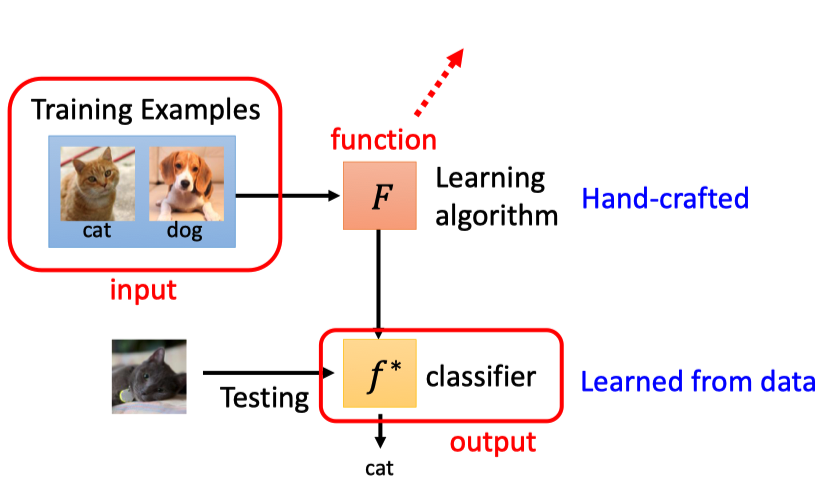
\includegraphics[width=1.0\textwidth]{figs/intro.png}}
	%\pause

	\textbf{But, can we learn the function F ? Or aka. Meta learning }

}
%%//////////////////////////////////////////////////////////////////////////////////////////////%%3
\frame{
	\frametitle{Introduction: Meta-Learning}

	\textbf{Meta learning = Learning to learn}

	* \ccr{Meta} + X $\longrightarrow$ X about X%\pause

	\centerline{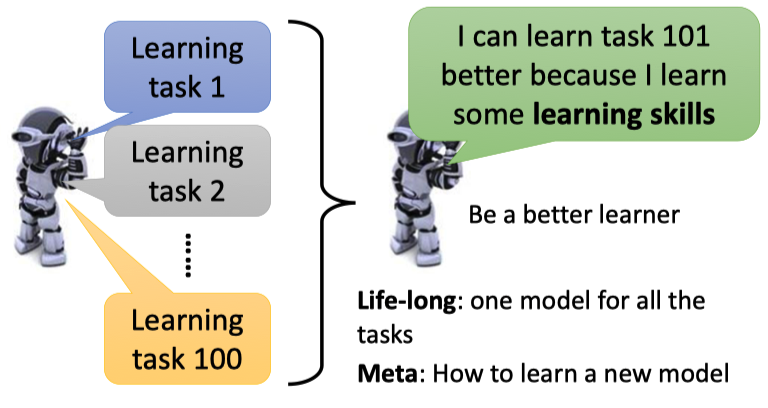
\includegraphics[width=1.0\textwidth]{figs/meta-ml.png}}
}
%%//////////////////////////////////////////////////////////////////////////////////////////////%%3
\frame{
	\frametitle{Introduction: Meta-Learning}

	\textbf{Define the goodness of function F}

	$ L(F) = sum_{n=1}^{N} l^n $

	\textbf{Find the best function F* according to L(F)}

	\centerline{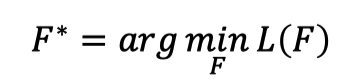
\includegraphics[width=1.0\textwidth]{figs/equation1.png}}

}
%%//////////////////////////////////////////////////////////////////////////////////////////////%%3
\frame{
	\frametitle{Introduction: Meta-Learning}
	\textbf{A Meta-Learning Model}
	\begin{itemize}
		\item learns from \ccb{past learning experience}		%\pause
		\item can learn \ccb{future tasks} \ccr{better} based on prior knowledge%\pause
		\item learns the learning function during the learning process
	\end{itemize}%\pause

	\textbf{Metrics for Meta-learning}
	\begin{itemize}
		\item size of training-set for model convergence	%\pause
		\item robustness of model %\pause
		\item accuracy of the prediction
		\item etc...
	\end{itemize}

}

%
%%//////////////////////////////////////////////////////////////////////////////////////////////%%13

\frame{
	\frametitle{Introduction: Start with Machine learning}
	\ccp{ Conventional supervised machine learning}
	\vspace{-2mm}
	\begin{itemize}
		\item  dataset  \ccb{$\mathcal{D} = {(x_1, y_1), . . . ,(x_N , y_N )}$} is given.
		\item \ccb{$(x_i, y_i)$}: pair of input data and output classification or regression result, such as (input image, output label).
		\item Predictive model: $\hat{y}=f_\theta(x)$, trained by $\theta^*=\arg \min_\theta \mathcal{L}(\mathcal{D};\theta,\omega)$.
	\end{itemize}\vspace{5mm}
	\centerline{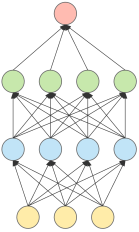
\includegraphics[width=0.1\textwidth]{figs/ml.png} $f($ 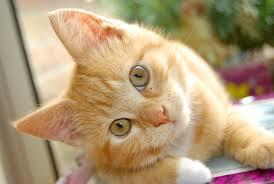
\includegraphics[width=0.2\textwidth]{figs/cat1.png} $) = ``cat"$}
}
%
%%//////////////////////////////////////////////////////////////////////////////////////////////%%13

\frame{
	\frametitle{Introduction: Problem triggered}
	\ccp{No enough dataset?}
	\vspace{-2mm}
	\begin{itemize}
		\item When there are enough samples for dataset $\mathcal{T}$, we can achieve ideal result. However, this may be difficult or even not possible.
		\item What if Alphago hadn't played Go for many times?
		\item How does Taobao recommend items to new user?
	\end{itemize}\vspace{3mm}
	\centerline{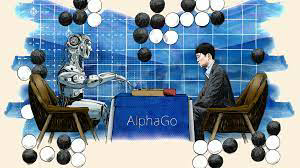
\includegraphics[width=0.3\textwidth]{figs/alphago.png} 
\includegraphics[width=0.2\textwidth]{figs/taobao.jpeg}}
	\vspace{-2mm}
	\begin{definition}
		\ccp{Few-shot learning} is the problem of making predictions based on a limited number of samples.
		\begin{itemize}
			\ccg{
			\item Few-shot classification: image classification, short text sentiment classification, and object recognition.
			\item Few-shot regression: cold-start recommendation.}
		\end{itemize}
	\end{definition}
}

%%%%//////////////////////////////////////////////////////////////////////////////////////////////%%14
%
\frame{
	\frametitle{Introduction: Meta learning}
	\vspace{-2mm}
	\ccp{Humans} vs \ccp{Machine}
	\begin{columns}
		\begin{column}{5cm}
			\begin{itemize}
				\item Children who have only seen trees and flowers a few times can distinguish them quickly.
				\item People able to ride a bike will most likely find a way to ride a motorcycle fast with little or even no demonstration.
			\end{itemize}
		\end{column}
		\begin{column}{5cm}
			\begin{itemize}
				\item  Inspired by human behaviors, The idea of meta learning is to design a model with an adaption process which happens during test but is exposed to the new task configurations properly.
			\end{itemize}
		\end{column}
	\end{columns}\vspace{5mm}
	\ccb{Solution}
	\vspace{-2mm}
	\begin{itemize}
		\item  learn from scratch $\rightarrow$  learn from a distribution of tasks $\mathcal{T}\sim p(\mathcal{T})$.
		\item algorithm function with $\omega$ pre-specified $  \rightarrow $ learn the learning algorithm.
		\item \ccb{learning to learn.}
	\end{itemize}\vspace{5mm}
}
%%%//////////////////////////////////////////////////////////////////////////////////////////////%%15

\frame{
	\frametitle{Introduction: Meta learning}
	\vspace{5mm}
	\begin{itemize}
		\item 	\ccp{Machine learning} $\approx $ The ability to find a function f according to the data.
		      \centerline{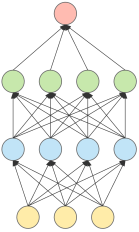
\includegraphics[width=0.1\textwidth]{figs/ml.png} $f($ 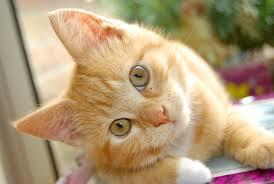
\includegraphics[width=0.2\textwidth]{figs/cat1.png} $) = ``cat"$}

		      \vspace{5mm}
		\item \ccp{Meta learning} $\approx $ According to the data, find the ability to find a function F of a function f.
		      \centerline{F(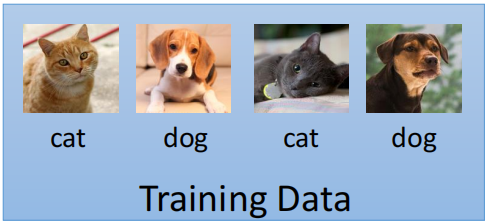
\includegraphics[width=0.4\textwidth]{figs/training_data.png}) = f* 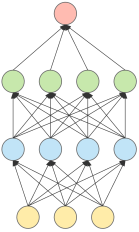
\includegraphics[width=0.1\textwidth]{figs/ml.png}}

	\end{itemize}
}

%%%%//////////////////////////////////////////////////////////////////////////////////////////////%%24

\section{MAML}

%%%%//////////////////////////////////////////////////////////////////////////////////////////////%%25

\frame{
	\frametitle{Model Agnostic Meta-Learning (MAML)}
	\begin{lemma}
		Let \ccb{$f$} be any flow and let \ccb{$(A,B)$} be any cut. Then, the value of the flow \ccb{$f$} equals the net flow across the cut \ccb{$(A,B)$}.
		\ccb{\begin{equation*}
				v a l(f)=\sum\limits_{\text { out of } A} f(e)-\sum\limits_{e \text { in to } A} f(e)
			\end{equation*}}
	\end{lemma}

	\bigskip
	\centerline{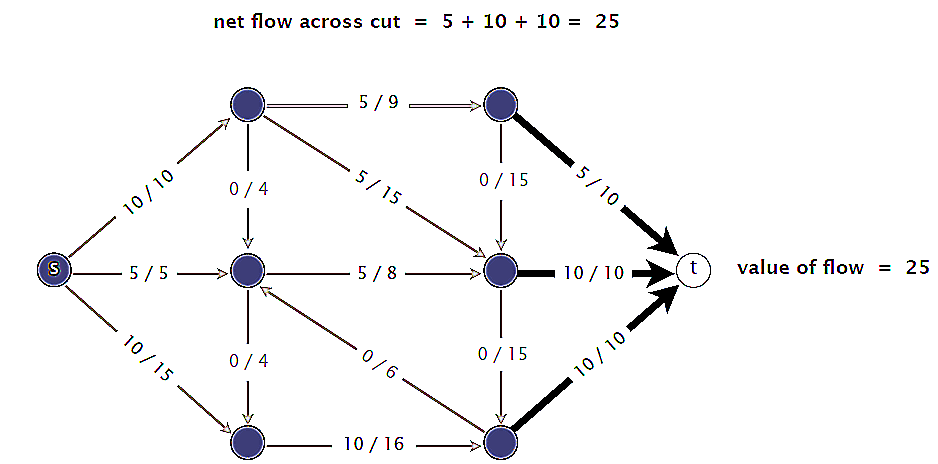
\includegraphics[width=0.8\textwidth]{figures/p25}}
}


%%//////////////////////////////////////////////////////////////////////////////////////////////%%36

\section{MeLU: MAML for Cold-Start Recommendation}

%%//////////////////////////////////////////////////////////////////////////////////////////////%%37
%%
%%
\frame{
	\frametitle{Cold-Start Recommendation problem}

	\ccp{Recommendation.} \\
	Companies use recommendation systems to deliver personalized contents and sell products.

	\begin{columns}
		\begin{column}{8cm}
			\centerline{
\includegraphics[width=0.3\textwidth]{figs/tiktok.png}}
		\end{column}
		\begin{column}{4cm}
			\centerline{
\includegraphics[width=0.3\textwidth]{figs/taobao.jpeg}}
		\end{column}
	\end{columns}
	%\pause

	\ccp{Cold-Start problem.} \\
	Modern recommendation systems use \ccp{Machine Learning} approach to provide \ccp{customized} user-experience.
	Recommendation using ML is hard when \#users and \#items are still small. (\ccr{A Cold-Start}).

	%\pause

	\begin{definition}
		\ccm{Few-Shot Learning}
		\begin{itemize}
			\item Few-shot learning is the problem of making predictions based on a limited number of samples.
		\end{itemize}
	\end{definition}
}

%%//////////////////////////////////////////////////////////////////////////////////////////////%%37

\frame{
	\frametitle{MAML for cold-start recommendation}

	\ccr{User Preference Estimator.} the model that estimate users' preference for certain item.
	\centerline{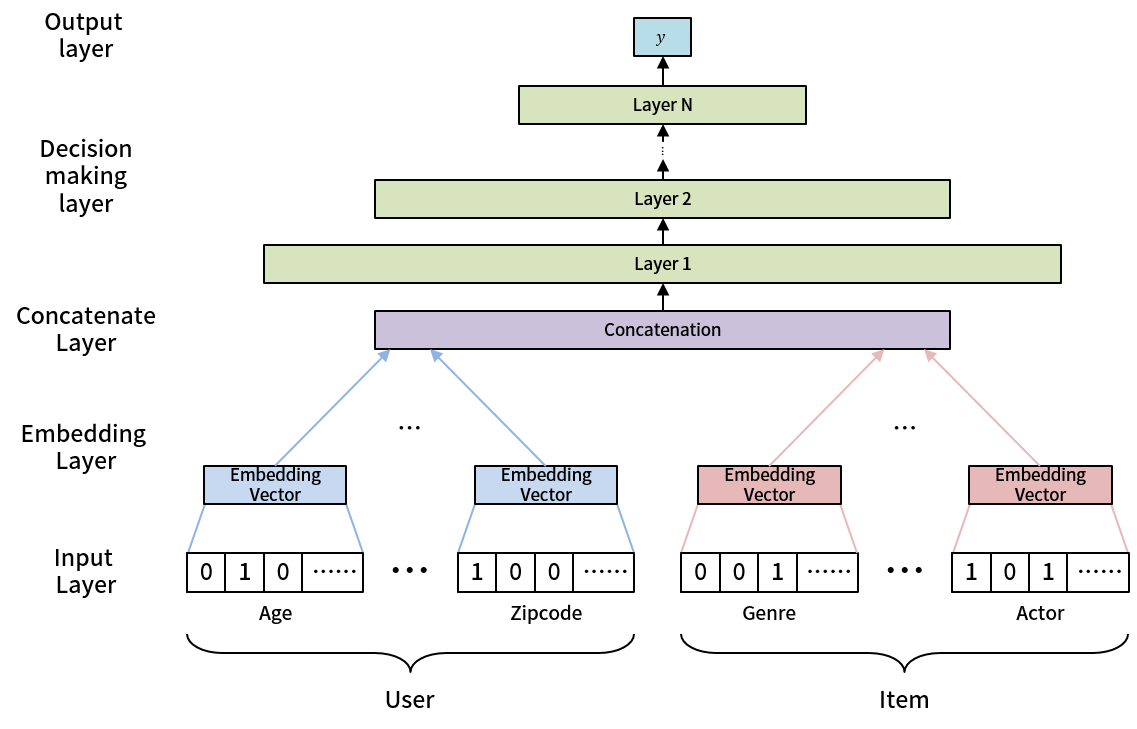
\includegraphics[width=1\textwidth]{figs/melu-pref.png}}

}
%%
%%%%//////////////////////////////////////////////////////////////////////////////////////////////%%38

\frame{
	\frametitle{User Preference Estimator.}

	\begin{block}{Model layers of UPE}
		\begin{itemize}
			\item \textbf{Input Layer} : get input information, including user's profile and item's information %\pause
			\item \textbf{Embedding Layer} : Embedding input information into embedding vectors. %\pause
			\item \textbf{Concatenate Layer}: Concatenate different vectors into one big vector. %\pause
			\item \textbf{Decision-Making Layers}: transform concatenated vector into characteristics  %\pause
			\item \textbf{Output Layer}: get output information in the form of preference probability, rating, dwell time,etc.
		\end{itemize}
	\end{block} %\pause

	This typical user preference estimator takes users' content and item content as input, and output preference prediction.
}

%%%%//////////////////////////////////////////////////////////////////////////////////////////////%%46

\frame{
	\frametitle{Meta-learned User Preference Estimator}

	\textbf{How to improve estimator's performance when \ccr{training set is small ?}}

	Apply MAML's approach to UPE ! %\pause

	\centerline{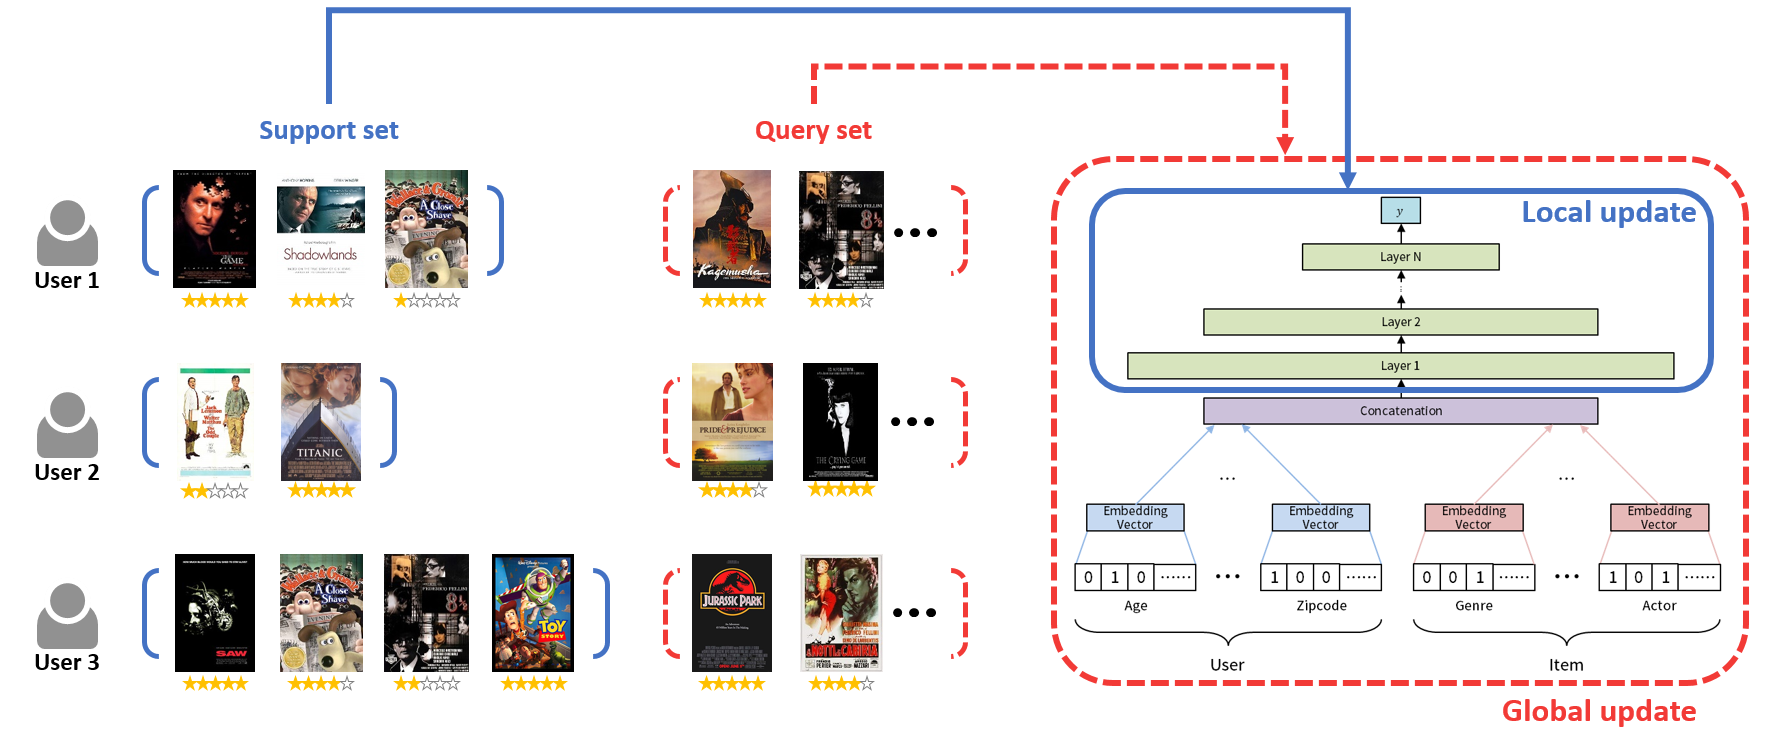
\includegraphics[width=1\textwidth]{figs/meta-upe.png}}

}

%%%%//////////////////////////////////////////////////////////////////////////////////////////////%%46

\frame{
	\frametitle{Meta-learned User Preference Estimator}

	\begin{block}{Loss function of UPE}
		$\mathcal{L}_i = \frac{1}{\left | H_i \right | } \sum_{j\in H_i} (y_{ij} - \hat{y}_{ij})^2 $
	\end{block} %\pause

	\centerline{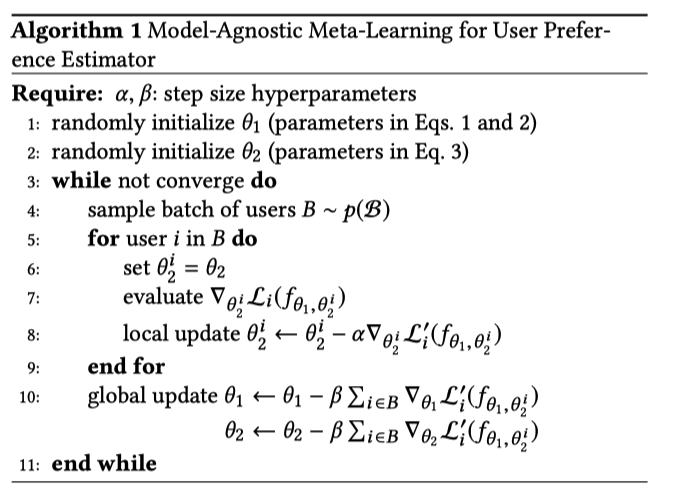
\includegraphics[width=0.8\textwidth]{figs/melu-alg.png}}
}

%%%%//////////////////////////////////////////////////////////////////////////////////////////////%%46

\frame{
	\frametitle{Evidence Candidate Selection}

	\begin{block}{Evidence Candidates}
		\ccr{Evidence candidate} is a set of items that are presented to a new user, so that the model can get a quick understand of user's general preference for products.
	\end{block} %\pause

	\textbf{We can user evidence candidates to}
	\begin{itemize}
		\item quickly understand user's preference by doing a survey on \ccb{evidence candidate}
		\item collaborate with Meta-learning approach to further improve few-shot accuracy.
	\end{itemize}
	\centerline{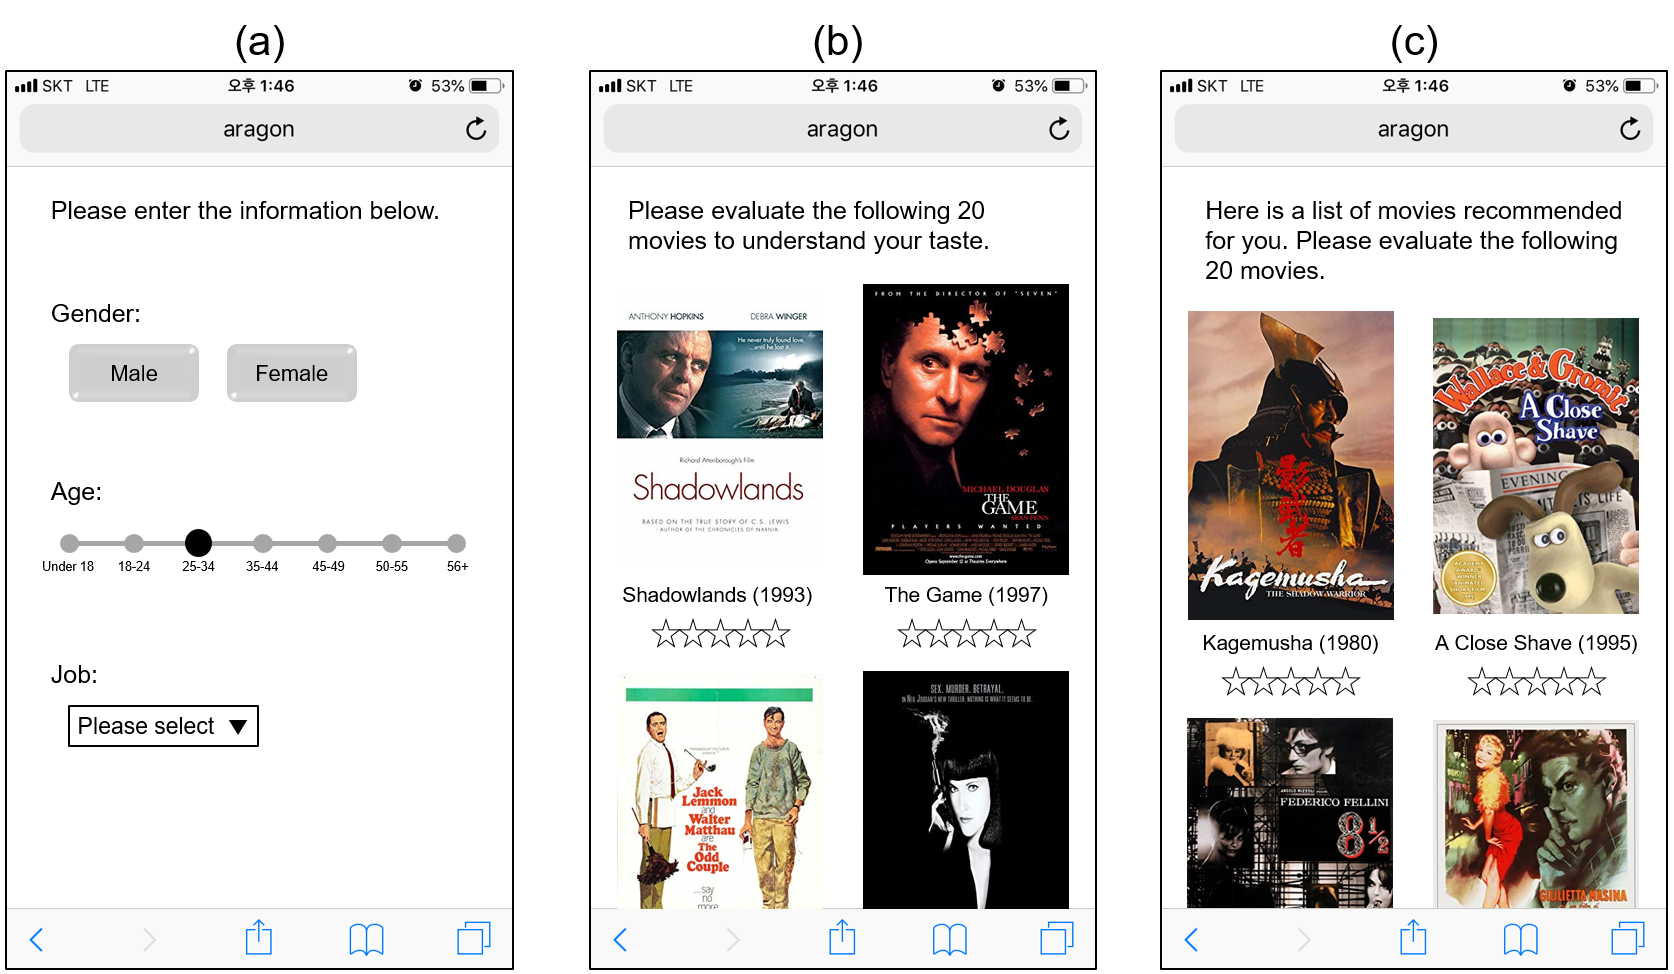
\includegraphics[width=0.5\textwidth]{figs/melu-candi.png}}

}

%%%%//////////////////////////////////////////////////////////////////////////////////////////////%%46

\frame{
	\frametitle{Evaluations}

	MeLU is able to predict well with only a few input.

	\textbf{The MAE of MeLU on the MovieLens and Bookcrossing datasets}
	\centerline{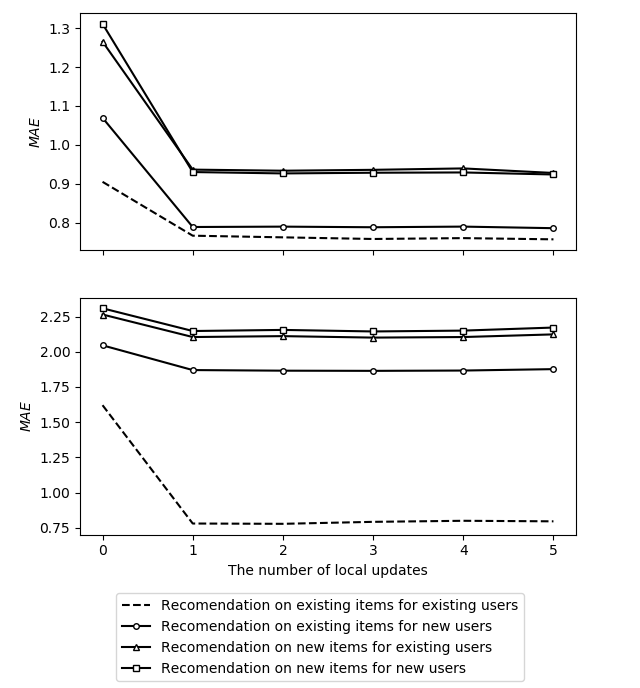
\includegraphics[width=1\textwidth]{figs/melu-eva.png}}

}
%%%%//////////////////////////////////////////////////////////////////////////////////////////////%%46

\frame{
	\frametitle{What can we learn from MeLU?}

	\textbf{MAML is a general approach}
	\begin{itemize}
		\item we can apply MAML to any gradient-based model.
		\item meta-learning approach can be useful in everyday tasks.
	\end{itemize}

	\textbf{Field-specific approach can be taken}
	\begin{itemize}
		\item to improve learning performance
		\item to focus on important metrics
	\end{itemize}


}
%%%%//////////////////////////////////////////////////////////////////////////////////////////////%% 7 pages

\section{More on meta-learning }

%%%%//////////////////////////////////////////////////////////////////////////////////////////////%%48
%%
\frame{
	\frametitle{Meta-learning is not only MAML}
	\textbf{MAML takes a optimization-based approach}
	\begin{itemize}
		\item MAML fundamentally produce a weight initialization, it learns a good initial parameter   %\pause
		\item not introduce any learned parameters more meta-learning  %\pause
		\item not actually learn any more general knowledge like \ccb{"how to learn a brand new task?"}
	\end{itemize} %\pause

	\textbf{There actually exists other approaches}
	\begin{itemize}
		\item Model-based : a new model designed specifically for fast learning, which in its nature updates parameters rapidly. May use RNN and memory techniques. %\pause
		\item Metric-based : derive problem-dependent good metrics, to facilitate problem solving.
	\end{itemize}

}


%%%%//////////////////////////////////////////////////////////////////////////////////////////////%% 3
%%
\frame{
	\frametitle{Beyond Gradient Descent}
	\textbf{How to meta-learn other metrics on models other than gradient-based.}

	\centerline{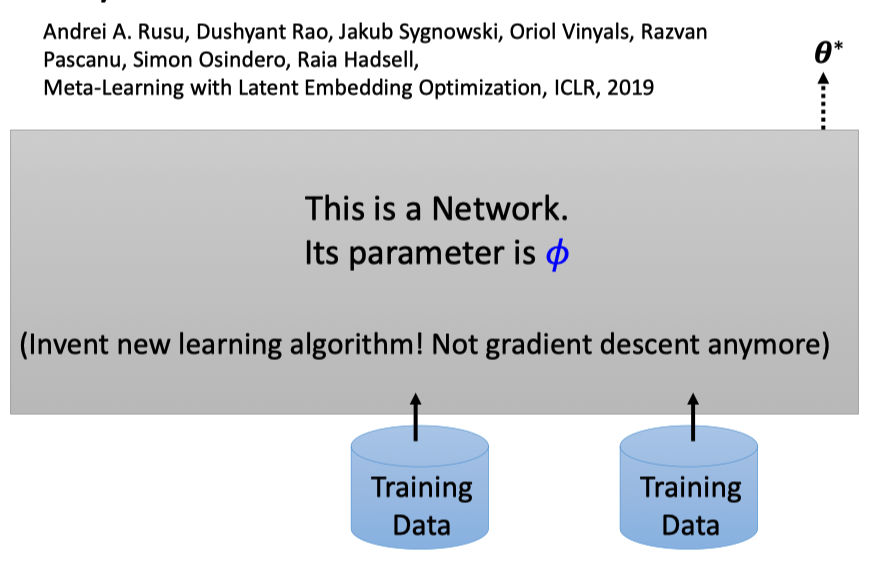
\includegraphics[width=1\textwidth]{figs/beyond-gd.png}}
}
%%%%//////////////////////////////////////////////////////////////////////////////////////////////%% 3
%%
\frame{
	\frametitle{Meta-learning is a huge field}
	\textbf{Matching network}
	Matching network is one of the \ccr{metric-based} meta-learning works that targeting k-shot classification problems.

	\centerline{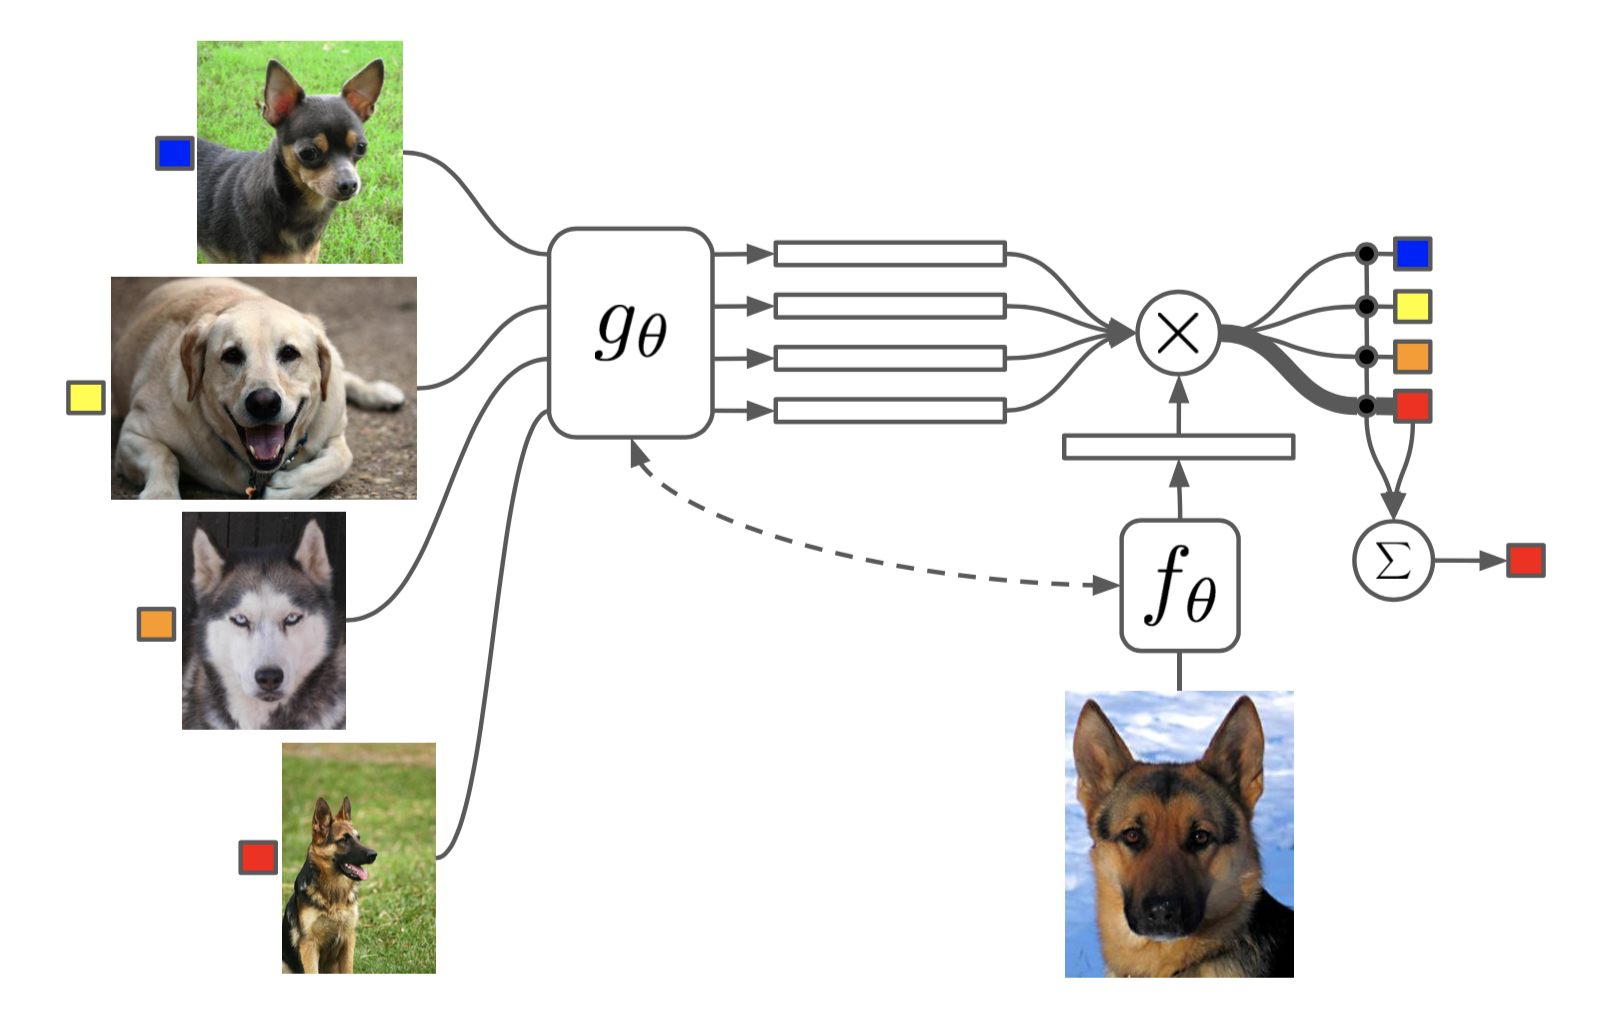
\includegraphics[width=1\textwidth]{figs/matching-networks.png}}
}

%%%%//////////////////////////////////////////////////////////////////////////////////////////////%% 3
%%
\frame{
	\frametitle{Meta-learning is a huge field}
	\textbf{Meta network}
	Meta Networks , short for MetaNet, is a \ccr{model-based} meta-learning model with architecture and training process designed for \ccpk{rapid generalization across tasks}.
	me
	\centerline{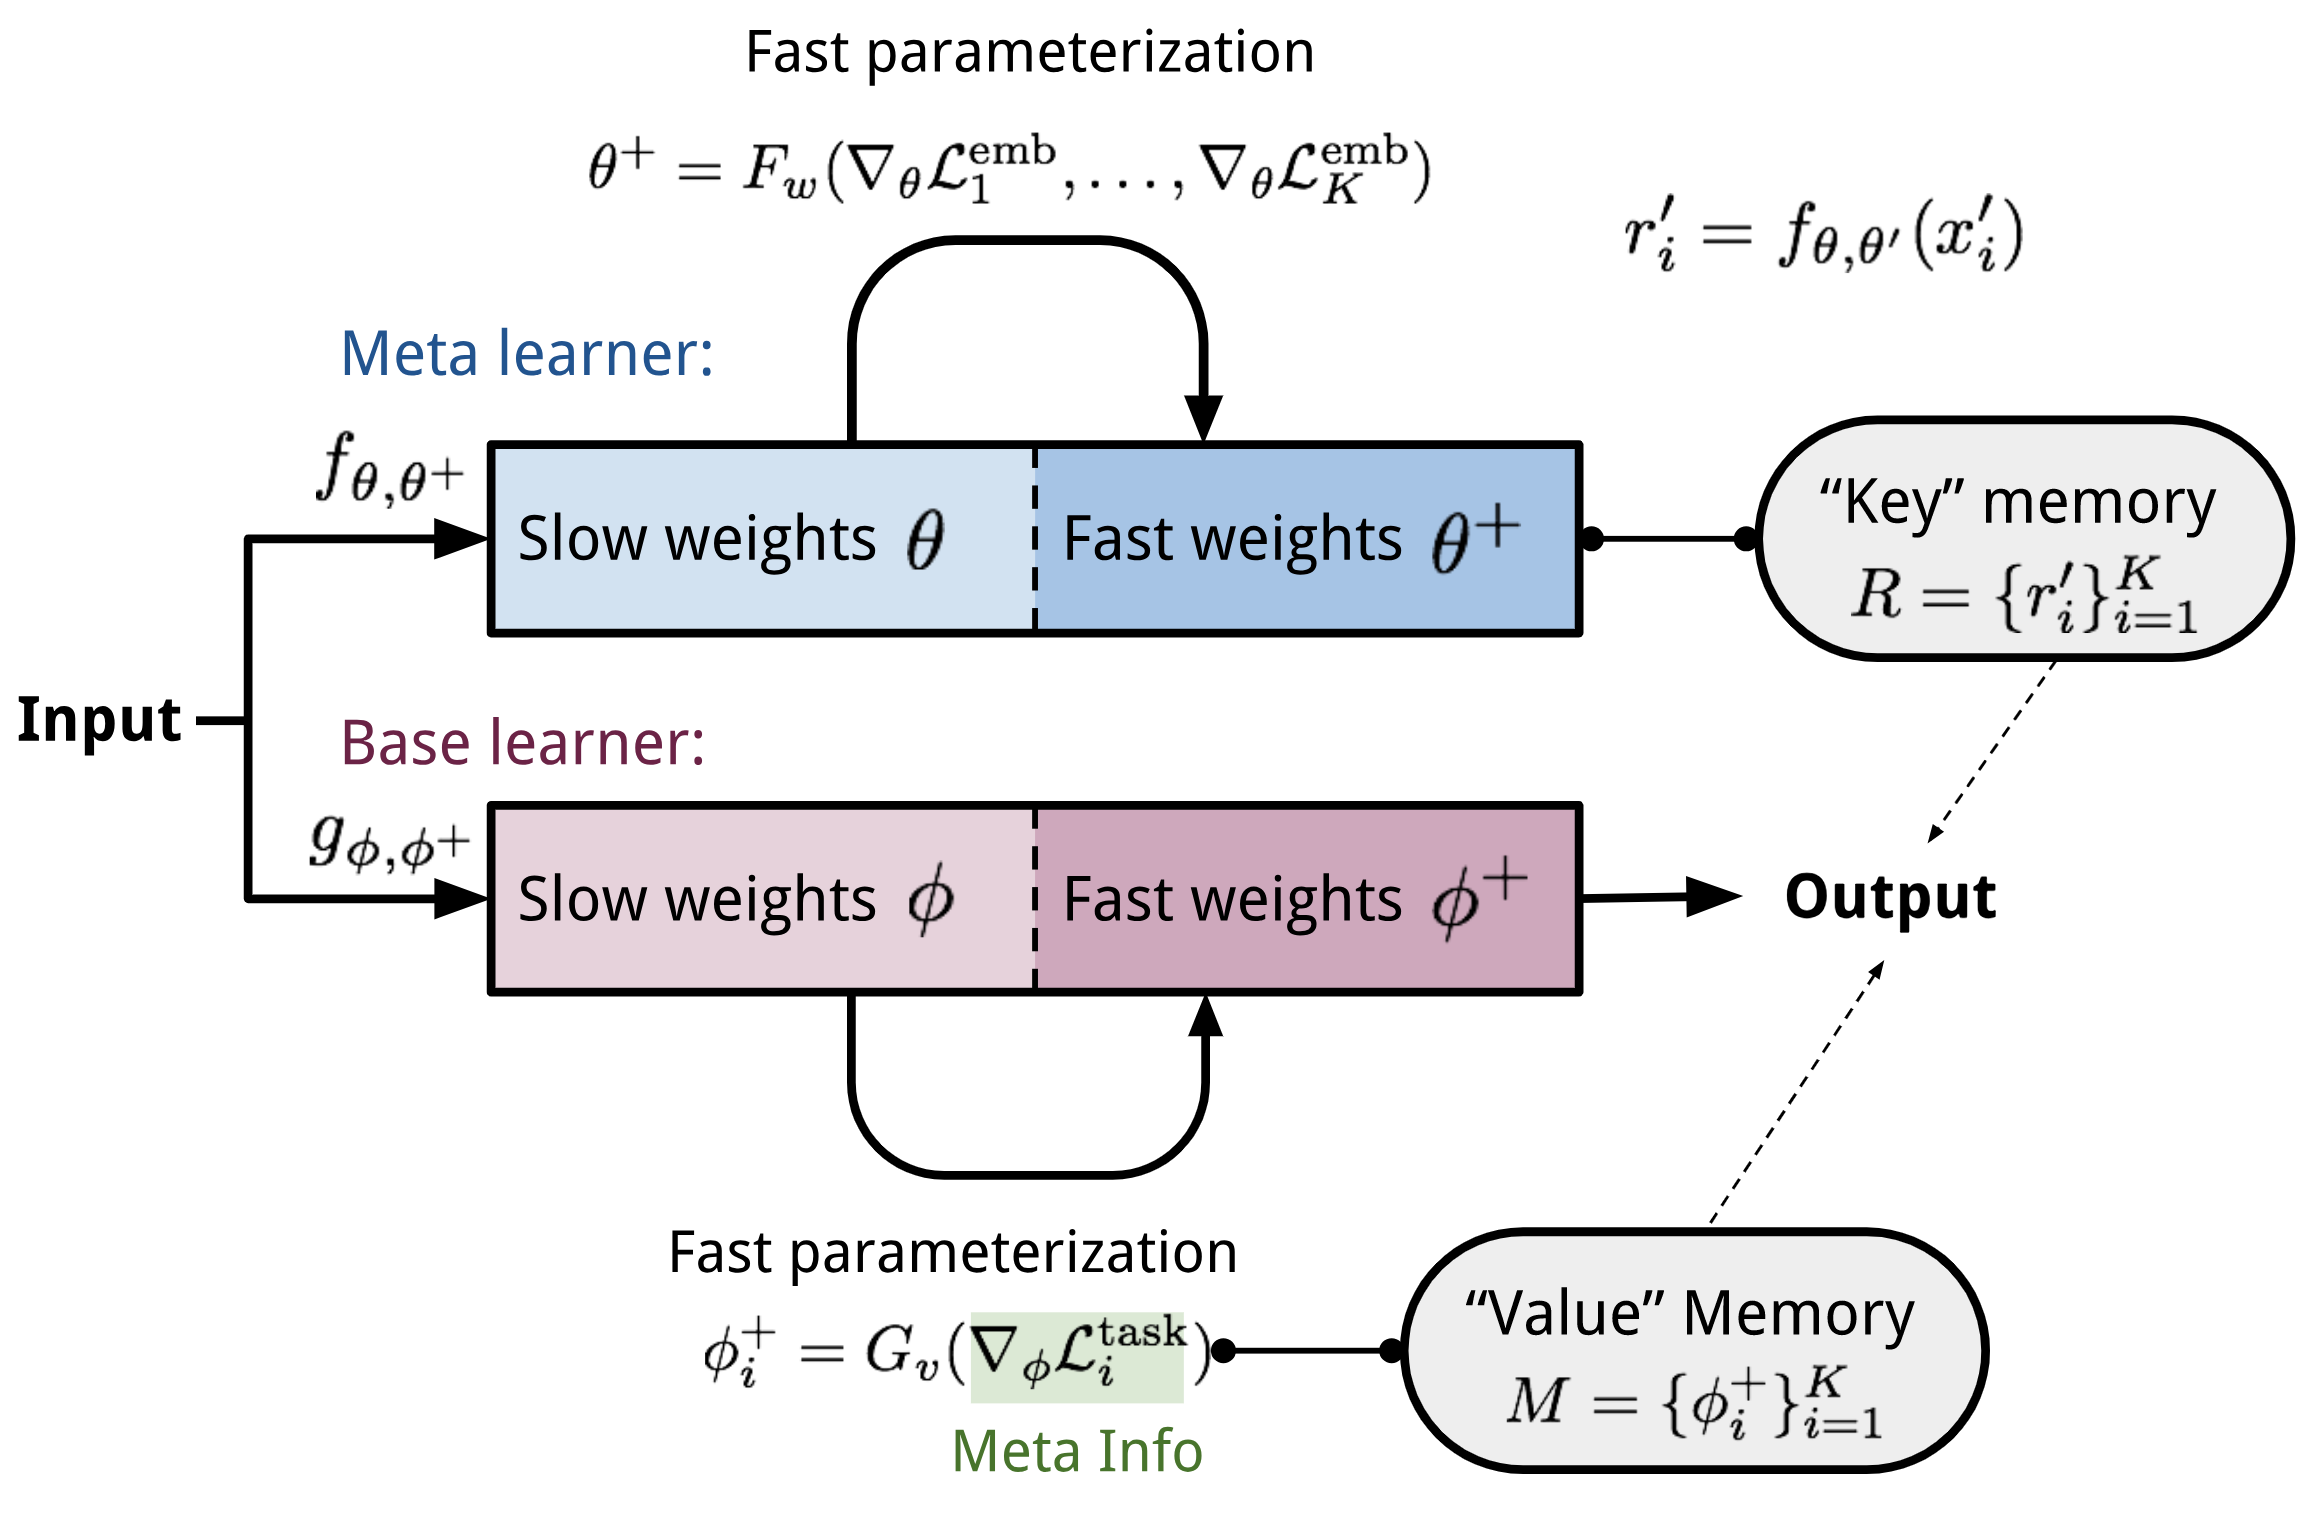
\includegraphics[width=1\textwidth]{figs/meta-network.png}}
}

%%%%//////////////////////////////////////////////////////////////////////////////////////////////%%48
%%
\frame{
	\frametitle{Meta-learning is a huge field}
	\textbf{Meta-learning Landscape}
	Overview of the meta-learning landscape including algorithm design (meta-optimizer, meta-representation, meta-objective), and applications.\\
	\ccg{from Hospedales. et al. "Meta-Learning in Neural Networks: A Survey." }

	\centerline{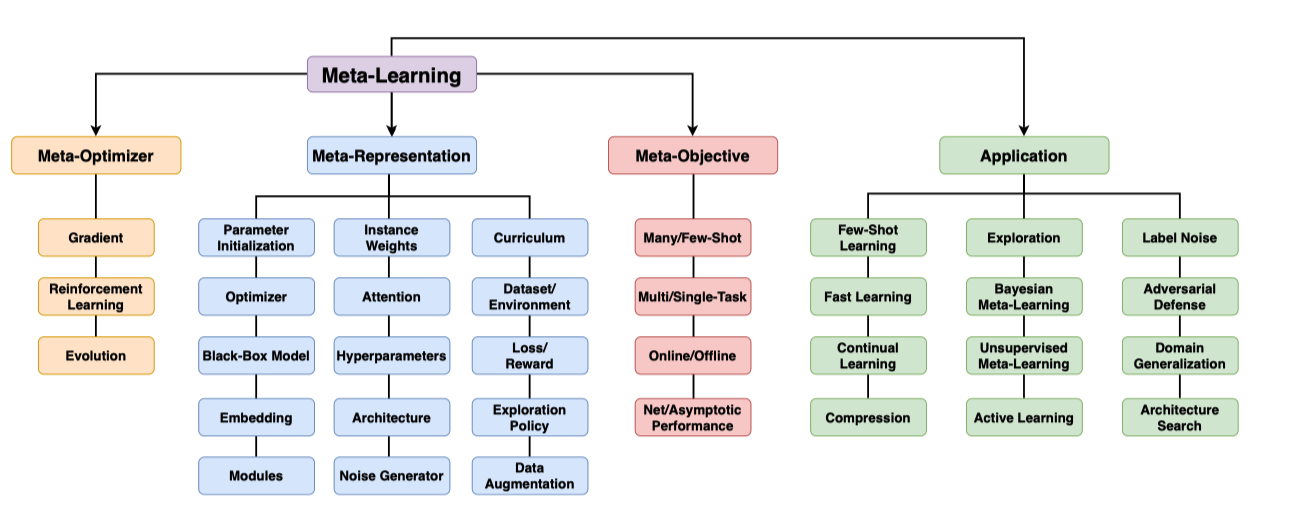
\includegraphics[width=1.1\textwidth]{figs/ml-landscape.png}}
}

%%//////////////////////////////////////////////////////////////////////////////////////////////%%58
\end{document}